%\section{Thesis Formatting Guidelines}

%This thesis template in Word document format was created to ensure that you will spend more time generating content for your paper and less time stressing about formatting issues. To ensure, however, that your document is truly formatted according to specifications, here are some formatting guidelines which you may use to evaluate your own paper’s formatting.

%\begin{enumerate}
%\item There should be NO PAGE NUMBERS on the first page of every chapter/section..
%\item Tables must have NO VERTICAL LINES, as well as NO INNER HORIZONTAL LINES after the table headers.
%\item Figures and tables are numbered ACCORDING TO CHAPTER NUMBER (e.g. Table 3.1 must be located in Chapter 3, and Figure B.2 is in Appendix B).
%\item The sequence of front matter must be as follows:
%    \begin{enumerate}
%    \item Title Page, in the correct formatting (e.g. Titles must be written in an inverted triangle, in ALL CAPS and boldface)
%    \item Abstract
%	\item Table of Contents
%	\item List of Figures
%	\item List of Tables
%	\end{enumerate}
%\item Upon binding, the front cover must contain the EXACT CONTENT AND FORMAT as that of your thesis’ title page.
%\end{enumerate}
\chapter{NUMERICAL APPROXIMATIONS}
Transcendental functions such as the exponential and logarithmic functions are usually implemented in computer hardware and software libraries using minimax polynomials, which are determined numerically using the Remez algorithm \cite{harrison_computation_1999}.
However, the Remez algorithm relies on iteratively refining the polynomial coefficients, which requires knowledge of the argument passed to the exponential or logarithmic function.

We cannot directly apply this approach in privacy-preserving image processing as we do not have knowledge of the exact value of the function arguments. In order to calculate a function under a  homomorphic cryptosystem, it is necessary to express the function in terms of the homomorphic operations.
In this section, we discuss approximations for the logarithm ($\log(1+x)$) and power ($x^r$) functions using only addition, subtraction, multiplication, and division operations.
.

%TODO: Explain why standard methods for transcedental function approximation cannot be applied here.
%TODO: Include citations for this chapter
\section{Approximation for $\log(1+x)$}
\label{sec:logapproximation}
We approximate the function $f(x)=\log(1+x)$ using a similar method to that described in
\cite{khattri_new_2009}.
We let $x = 1/n$ and consider the integral
\begin{align*}
  \int_{n}^{n+1}{\frac{1}{x}\diff x}=\log{\left(1+\frac{1}{n}\right)}.
\end{align*}
This integral can be approximated using the five-point Gauss-Legendre quadrature rule \cite{kythe_quadrature_2002}, which is as follows:
\begin{align*}
	\int_a^b{f(x)\diff x}
	&= \frac{b-a}{2}\int_{-1}^{1}{f\left(\frac{b-a}{2}x+\frac{a+b}{2}\right)\diff x}\\
	\int_{-1}^{1}{f(x)\diff x} &= \sum_{i=1}^{5}{w_if(x_i)}
\end{align*}
where
\begin{multicols}{2}
	\noindent
	\begin{align*}
		w_1 &= 0\\
		w_2 &= \frac{1}{21}\sqrt{245-14\sqrt{70}}\\
		w_3 &= -\frac{1}{21}\sqrt{245-14\sqrt{70}}\\
		w_4 &= \frac{1}{21}\sqrt{245+14\sqrt{70}}\\
		w_5 &= -\frac{1}{21}\sqrt{245+14\sqrt{70}}\\
	\end{align*}
	\columnbreak
	\begin{align*}
		x_1 &= \frac{128}{225}\\
		x_2 &= \frac{1}{900}\left( 322 + 13\sqrt{70}\right)\\
		x_3 &= \frac{1}{900}\left( 322 + 13\sqrt{70}\right)\\
		x_4 &= \frac{1}{900}\left( 322 - 13\sqrt{70}\right)\\
		x_5 &= \frac{1}{900}\left( 322 - 13\sqrt{70}\right)\\
	\end{align*}
\end{multicols}
This yields the following approximation:
\begin{equation}\label{eq:standardquadrature}
  \log(1+x) =
  \frac{137x^5 + 2310x^4 + 9870x^3 + 15120x^2 + 7560x}
  {30x^5 + 900x^4 + 6300x^3 + 16800x^2 + 18900x + 7560}.
\end{equation}
While this closed form approximation is accurate for values of $x$ near zero, it diverges from $\log{(1+x)}$ significantly for large values of $x$.
\begin{figure}[!ht]
    \centering
    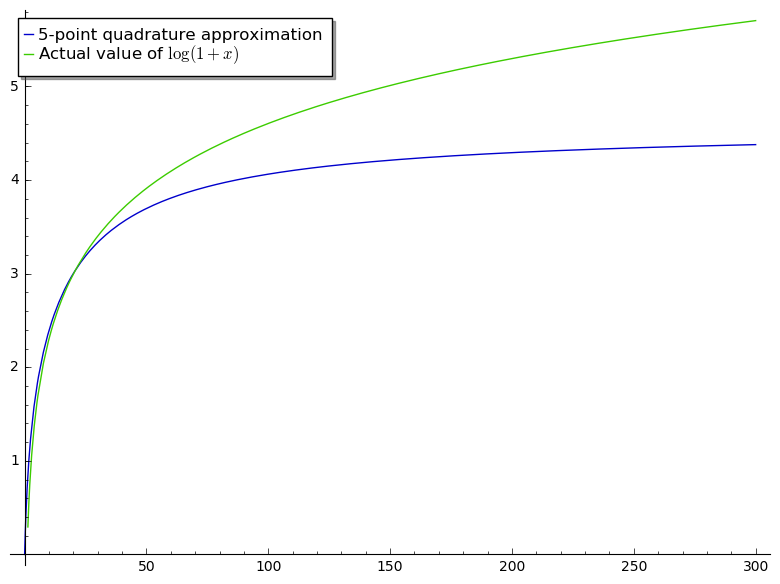
\includegraphics[width=.6\linewidth,\keepaspectratio]{figures/StandardQuadrature.png}
    \caption{Graph of $\log{(1+x)}$ and the approximation in equation \ref{eq:standardquadrature}}
    \label{fig:standardquadrature}
\end{figure}
As we only need accuracy for $x \in [0, 255]$, we can scale the approximation by a constant factor $\alpha$ as follows:
\begin{align*}
  \log{(1+x)} &= \log{\left(\frac{\alpha + \alpha x}{\alpha}\right)}\\
  &= \log{(\alpha + \alpha x)} - \log{\alpha}\\
  &= \log{\left(\alpha+\frac{\alpha}{n}\right)} - \log{\alpha}\\
  &= \log{\left(\frac{\alpha n + \alpha}{n}\right)} - \log{\alpha}\\
  &= \int_{n}^{\alpha n + \alpha}{\frac{1}{x}\diff x} - \log{\alpha}
\end{align*}

Using the five-point Gauss-Legendre quadrature rule with $\alpha = 1/20$, we arrive at the approximation:
\begin{align}\label{eq:scaledquadrature}
  \begin{split}
    &\log(1+x) \\
    &=\frac{137x^5 + 33185x^4 + 931370x^3 - 13403630x^2 - 289469315x - 713567363}
    {30(x^5 + 505x^4 + 42010x^3 + 923010x^2 + 5722005x + 8040501)} + \log{20}
  \end{split}
\end{align}
Below is a graph of the absolute error of the scaled approximation and the exact value of $\log{(1+x)}$.
\begin{figure}[!ht]
    \centering
    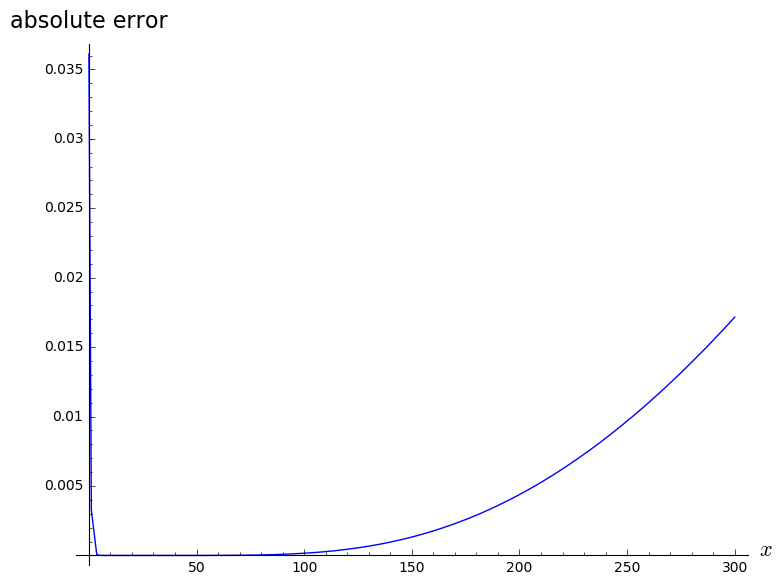
\includegraphics[width=.9\linewidth,\keepaspectratio]{figures/ModifiedQuadratureAbsoluteError.png}
    \caption{Graph of the absolute error of $\log{(1+x)}$ and the approximation in equation \ref{eq:scaledquadrature}}
    \label{fig:scaledquadrature}
\end{figure}
\section{Approximation for $x^\gamma$}
To approximate $x^\gamma$ for any $\gamma \in \mathbb{R}$, we rewrite $x^\gamma$ as follows:
\begin{align*}
  x^\gamma = e^{\log{x^\gamma}} = e^{\gamma\log{x}}.
\end{align*}
This expression can then be approximated using the Maclaurin series expansion for $e^x$, which converges for all $x$.
\begin{align*}
  e^x &= \sum_{n=0}^{\infty}{\frac{x^n}{n!}}\\
  \Rightarrow e^{\gamma\log{x}} &= \sum_{n=0}^{\infty}{\frac{(\gamma\log{x})^n}{n!}}
\end{align*}
As we already have an approximation for the natural logarithm, we can evaluate partial sums of the above infinite series to arrive at approximations for $x^\gamma$.
